\chapter{Zadatak 2}

U ovom dijelu zadatka je potrebno identificirati parametre stvarnog sistema opisanog funkcijom G(s) u koju su uvrštene vrijednosti a=2 i b=2.
	\[G(s)=\frac{0.16s+0.8}{s(60s^3+96s^2+39s+3)}\]
Identifikaciju je potrebno uraditi analizom odziva na impulsnu pobudnu funkciju (dobit ćemo odziv na step, a nakon toga dodati integrator u aproksimirani sistem) te aproksimirati dati sistem sistemom prvog reda sa čistim transportnim kašnjenjem $G_{ident} (s)$.
	\[G_{ident} (s)=\frac{1}{s}  \frac{k_{ob}}{T_{ob} s+1} e^{-\tau_ob s}\]
 

Na osnovu odziva na jediničnu pobudnu funkciju koji je skiciran na slici \ref{fig:z1_1}, određuju se parametri prenosne funkcije $G_{ident} (s)$ na način kako je opisano u prvom zadatku. 

Provedbom opisanog postupka u MATLAB-u dobivena je sljedeća prenosna funkcija:
	\[G_{ident} (s)=\frac{1}{s}  \frac{0.2667}{15.45s+1} e^{-1.74s}\]

Sada će biti prikazan step odziv (slika \ref{fig:z2_2}), impulsni odziv (slika \ref{fig:z2_3}), Bode dijagrami (slika \ref{fig:z2_4}) te raspored nula i polova (slika \ref{fig:z2_5}) stvarnog i aproksimiranog sistema.

\begin{figure} [H]
  \centering
  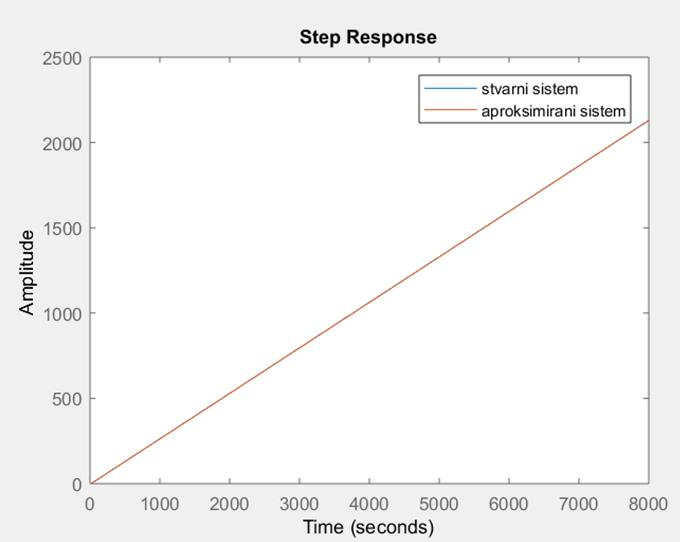
\includegraphics[width=0.8\textwidth]{z2_2}
  \caption{Identifikacija: odzivi sistema na step}
  \label{fig:z2_2}
\end{figure}

\begin{figure} [H]
  \centering
  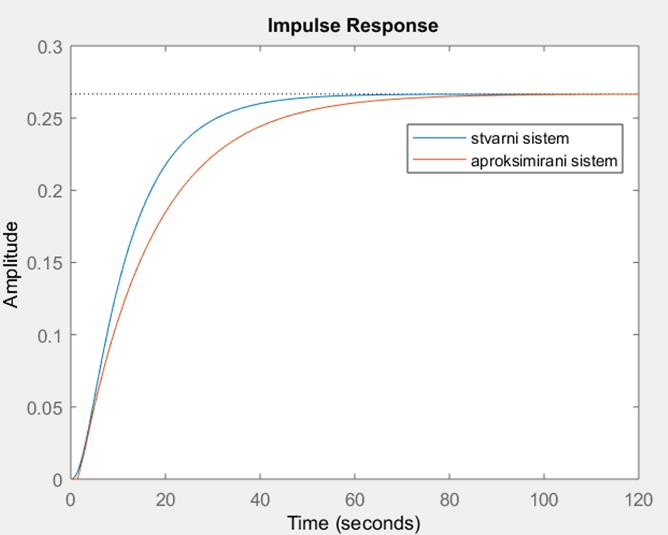
\includegraphics[width=0.8\textwidth]{z2_3}
  \caption{Identifikacija: impulsni odzivi sistema}
  \label{fig:z2_3}
\end{figure}

\begin{figure} [H]
  \centering
  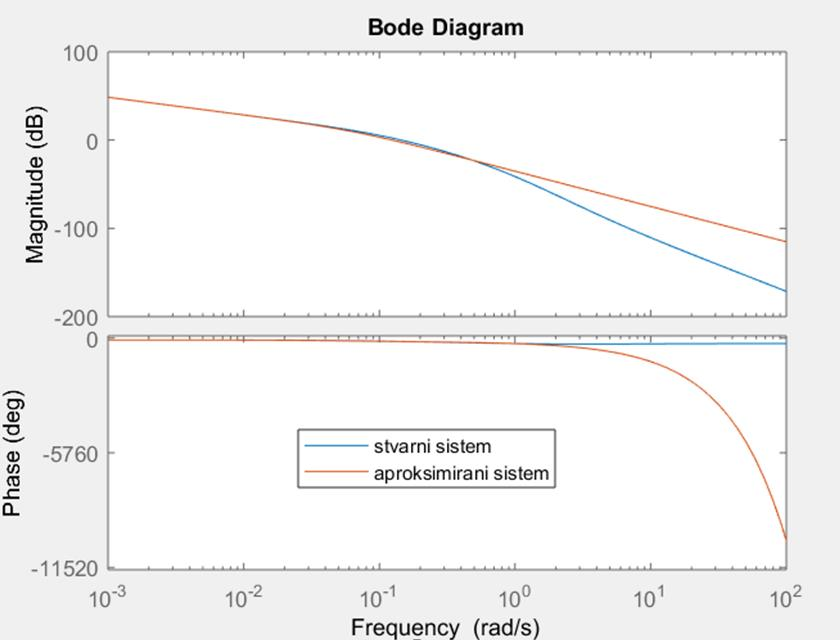
\includegraphics[width=0.8\textwidth]{z2_4}
  \caption{Identifikacija: Bode dijagrami sistema}
  \label{fig:z2_4}
\end{figure}
 
 \begin{figure} [H]
  \centering
  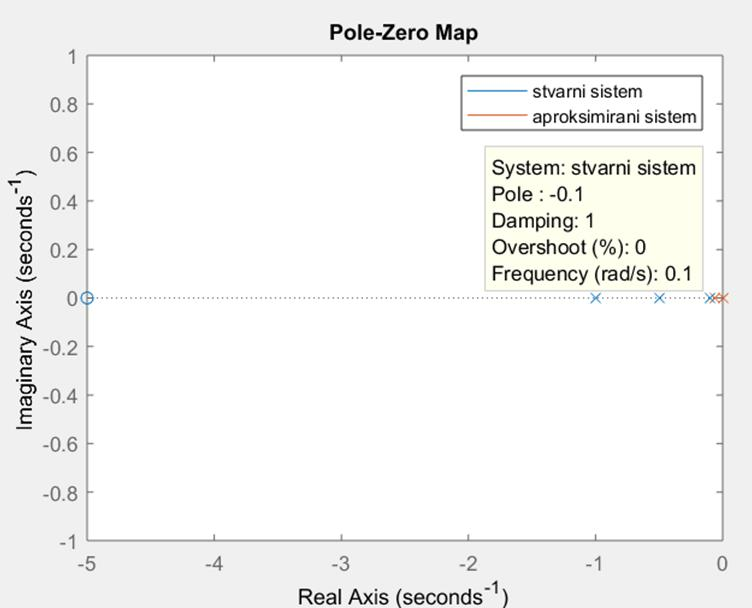
\includegraphics[width=0.8\textwidth]{z2_5}
  \caption{Identifikacija: polovi i nule sistema}
  \label{fig:z2_5}
\end{figure}

Možemo primijetiti da sistem prvog reda sa čistim transportnim kašnjenjem ima eksponencijalno opadajuću fazu (zbog logaritamske razmjere), tj. ima linearnu fazu zbog elementa transportnog kašnjenja. Što se tiče amplitudne karakteristike, i jedan i drugi sistem se ponašaju kao niskopropusni filteri, jedina je razlika što zbog reda sistema nakon prelomne frekvencije stvarni sistema ima jače slabljenje viših frekvencija zbog većeg reda sistema. Stvarni sistem je sistem 4. reda koji ima 4 pola. Dva konjugovano kompleksna pola su dominantna, ali zbog blizine nule njihov utjecaj slabi. Pol sistema prvog reda sa transportnim kašnjenjem je postavljen tako da aproksimira dinamiku sistema 4. reda, a postavljen je blizu dominantnog pola stvarnog sistema 4. reda, tj. blizu koordinatnog početka. Također, u aproksimiranom sistemu smo dodali pol u koordinatnom početku zbog postojanja astatizma u stvarnom sistemu. Ostali polovi imaju slabiji utjecaj na odziv sistema 4. reda pa je ova aproksimacija sistemom prvog reda sa čistim transportnim kašnjenjem dobra aproksimacija. Međutim, kako je odziv na step sistema sa astaizmom nestabilan u otvorenom (rampa je nestabilan signal), onda je potrebno prvo ustabiliti naš sistem, a nakon toga primijeniti regulaciju. To ćemo uraditi zatvaranjem jedinične negativne povratne sprege, uključujući pojačanje K=0.1. Tako dobivamo prenosnu funkciju:
	\[G_1 (s)=\frac{KG(s)}{1+KG(s)} =\frac{0.96s^4+6.336s^3+8.304s^2+3.168s+0.24}{3600s^7+11520s^6+13896s^5+7849s^4+2103s^3+242.3s^2+12.17s+0.24}\]
Prenosnu funkciju $G_1 (s)$ ćemo sada posmatrati kao naš sistem koji je potrebno aproksimirati metodama obrađenim u prvom zadatku. Identifikaciju je potrebno uraditi analizom odziva na jediničnu pobudnu funkciju te aproksimirati dati sistem sistemom prvog reda sa čistim transportnim kašnjenjem $G_{ident} (s)$. Ovo je urađeno prema proceduri objašnjenoj u prvom zadatku. Provedbom opisanog postupka u MATLAB-u dobivena je sljedeća prenosna funkcija:
	\[G_{ident} (s)=\frac{1}{49.58s+1} e^{-8.5s}\]

Sada će biti prikazan step odziv (\ref{fig:z2_6}), impulsni odziv (\ref{fig:z2_7}), Bode dijagrami (\ref{fig:z2_8}) te raspored nula i polova (\ref{fig:z2_9}) stvarnog i aproksimiranog sistema.

\begin{figure} [H]
  \centering
  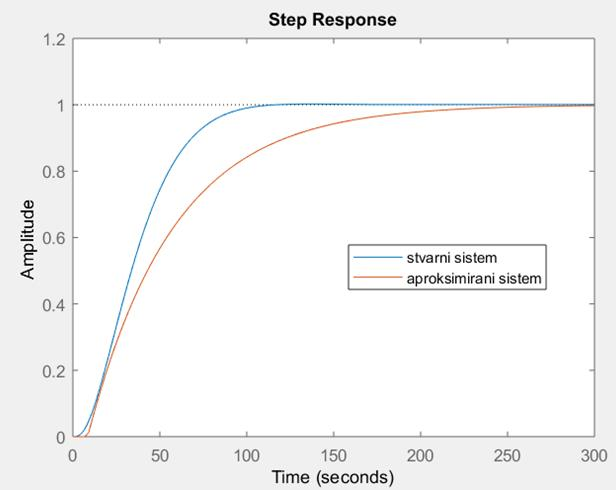
\includegraphics[width=0.8\textwidth]{z2_6}
  \caption{Identifikacija: odzivi sistema na step}
  \label{fig:z2_6}
\end{figure}

\begin{figure} [H]
  \centering
  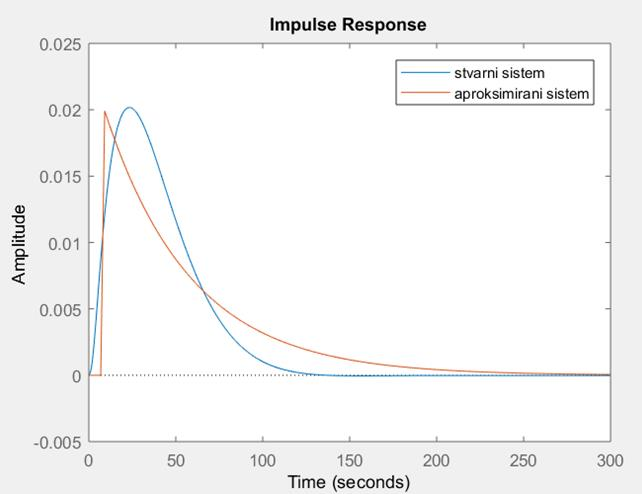
\includegraphics[width=0.8\textwidth]{z2_7}
  \caption{Identifikacija: impulsni odzivi sistema}
  \label{fig:z2_7}
\end{figure}

\begin{figure} [H]
  \centering
  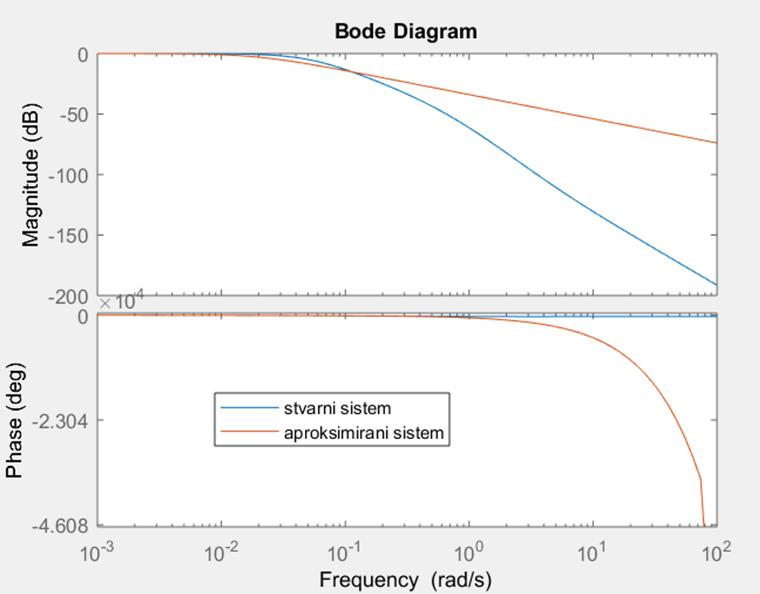
\includegraphics[width=0.8\textwidth]{z2_8}
  \caption{Identifikacija: Bode dijagrami sistema}
  \label{fig:z2_8}
\end{figure}
 
 \begin{figure} [H]
  \centering
  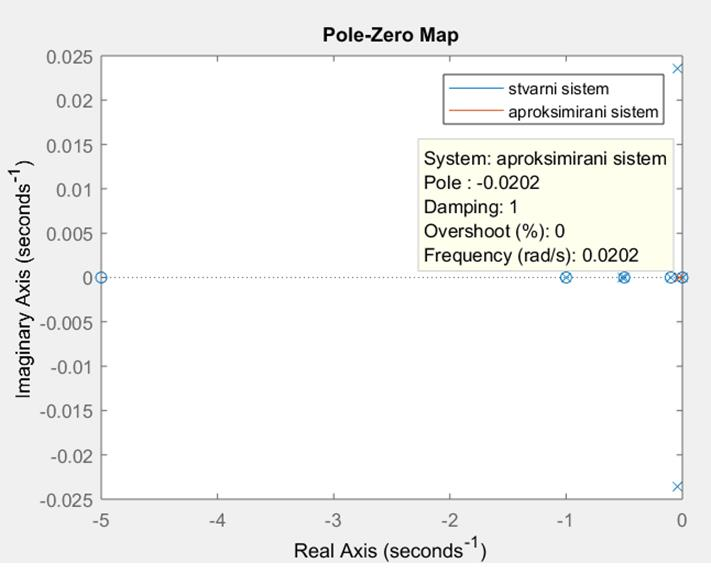
\includegraphics[width=0.8\textwidth]{z2_9}
  \caption{Identifikacija: polovi i nule sistema}
  \label{fig:z2_9}
\end{figure}

Možemo primijetiti da sistem prvog reda sa čistim transportnim kašnjenjem ima eksponencijalno opadajuću fazu (zbog logaritamske razmjere), tj. ima linearnu fazu zbog elementa transportnog kašnjenja. Što se tiče amplitudne karakteristike, i jedan i drugi sistem se ponašaju kao niskopropusni filteri, jedina je razlika što zbog reda sistema nakon prelomne frekvencije stvarni sistema ima jače slabljenje viših frekvencija zbog većeg reda sistema. Stvarni sistem je sistem 7. reda koji ima 7 polova. Dva konjugovano kompleksna pola su dominantna, ali zbog blizine nule njihov utjecaj slabi. Pol sistema prvog reda sa transportnim kašnjenjem je postavljen tako da aproksimira dinamiku sistema 7. reda, a postavljen je blizu dominantnog pola stvarnog sistema 7. reda.
Ostali polovi imaju slabiji utjecaj na odziv sistema 7. reda pa je ova aproksimacija sistemom prvog reda sa čistim transportnim kašnjenjem dobra aproksimacija.

\textbf{b)} U ovom dijelu će biti pokazani regulacioni krugovi napravljeni u Simulink-u za potrebe testiranja PID regulatora za aproksimirani i stvarni sistem (\ref{fig:z2_10}).
 
 \begin{figure} [H]
  \centering
  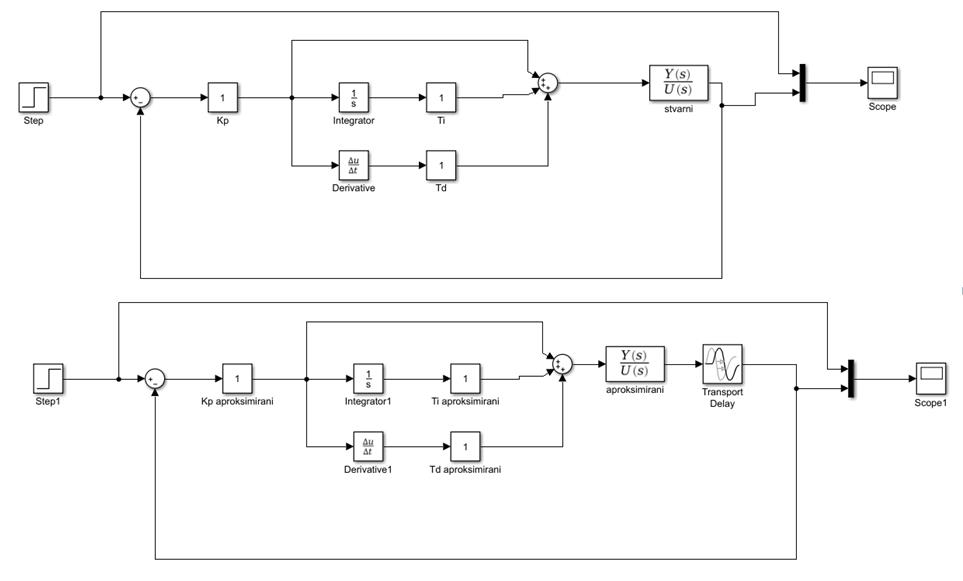
\includegraphics[width=0.8\textwidth]{z2_10}
  \caption{Regulacioni krugovi u Simulink-u u kojima je moguće varirati parametre PID regulatora za stvarni i aproksimirani sistem}
  \label{fig:z2_10}
\end{figure}


\textbf{c)} Povećanjem pojačanja $K_p$ postižemo brži odziv (slika \ref{fig:z2_11}). Također, u tom slučaju dolazi do smanjenja greške u stacionarnom stanju koju ipak nije moguće otkloniti kada koristimo samo P regulator jer kada bi greška postala jednaka nuli, tada ne bi bilo nikakvog djelovanja na sistem. To znači da će greška u stacionarnom stanju kod P regulatora uvijek postojati. Također, povećanjem pojačanja $K_p$ možemo učiniti sistem nestabilnim.

\begin{figure} [H]
  \centering
  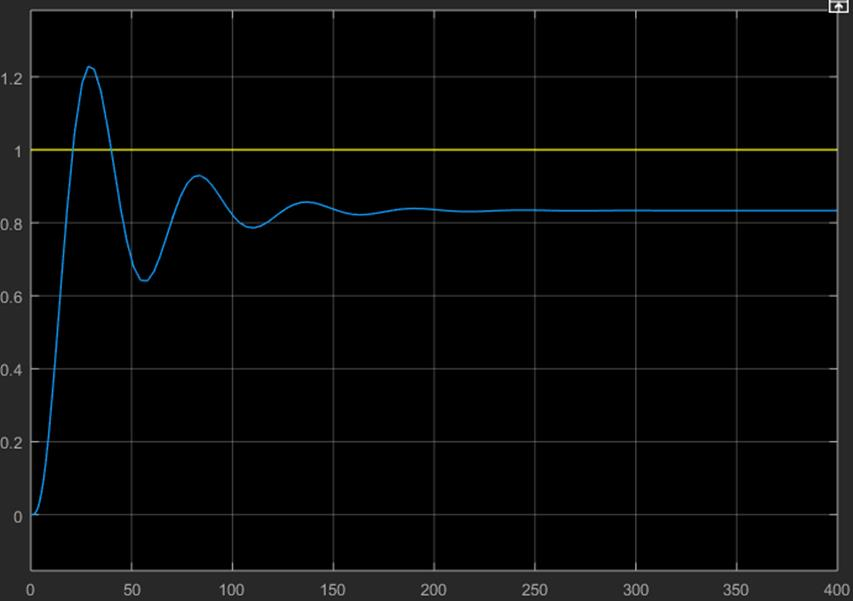
\includegraphics[width=0.8\textwidth]{z2_11}
  \caption{Odziv stvarnog sistema za $K_p=5$}
  \label{fig:z2_11}
\end{figure}

Dodavanjem djelovanja integralne komponente (slika \ref{fig:z2_12}) postižemo eliminisanje greške u stacionarnom stanju. Međutim, dolazi do većeg preskoka i povećanja vremena smirenja jer je došlo do oscilacija. Vrijeme porasta se smanjuje jer će integralna komponenta na početku generisati dodatno pojačanje u sistem sumiranjem pozitivne greške (greška kada se oduzmu zadana i trenutna vrijednost koja kreće iz nule).

\begin{figure} [H]
  \centering
  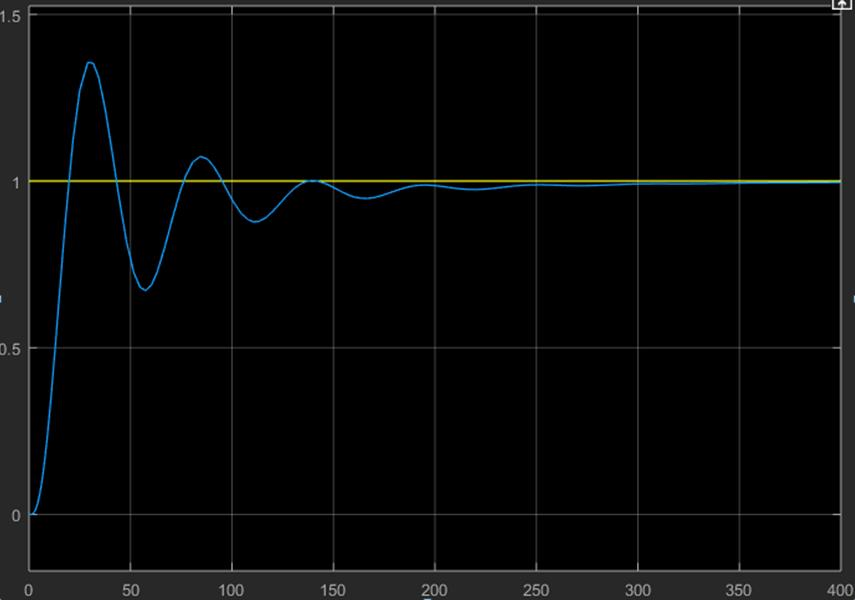
\includegraphics[width=0.8\textwidth]{z2_12}
  \caption{Odziv stvarnog sistema za $K_p=5, T_i=100$}
  \label{fig:z2_12}
\end{figure}

Sada je potrebno dovesti sistem u nestabilno stanje, a zatim primijeniti D komponentu PID regulatora. Izabrano je $T_i=10$ jer je tada sistem nestabilan.

\begin{figure} [H]
  \centering
  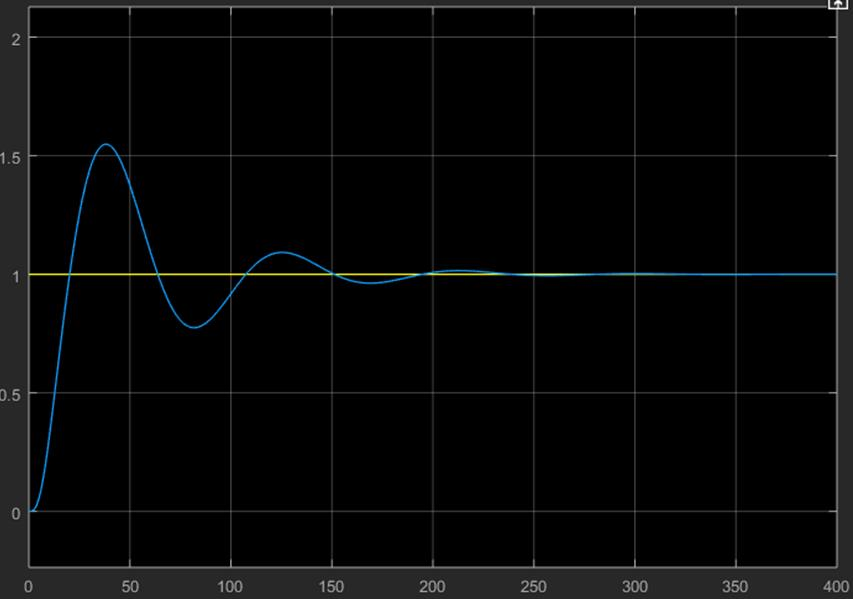
\includegraphics[width=0.8\textwidth]{z2_13}
  \caption{Odziv stvarnog sistema za $K_p=5, T_i=10, T_d=15$}
  \label{fig:z2_13}
\end{figure}
 
Dodavanjem D komponente (slika \ref{fig:z2_13}) PID regulatora sistem ponovo postaje stabilan. Dakle, P i I komponentu možemo još više pojačati za razliku od PI regulatora. Također, D komponetna povećava rezerve stabilnosti tako da je moguće sistem ustabiliti ukoliko je bio nestabilan (što je ovdje slučaj). D komponenta također smanjuje prvi preskok jer kaže kontroleru ako počne brzo da raste da uspori odziv, i obrnuto. Također, D komponenta smanjuje oscilacije u sistemu pa zbog toga smanjuje vrijeme smirenja.

\textbf{d)} Da bi izračunali kritično pojačanje $k_{krit}$ analitički, potrebno je da riješimo jednačinu:
	\[1+KG(s)=0\]

Povećavamo pojačanje od nule ka većim vrijednostima sve dok ne dobijemo da je jedno ili više rješenja ove jednačine čisto imaginarno, a ostala rješenja sa realnim dijelom manjim od nule. Tada je sistem na granici stabilnosti. Pojačanje za koje dobijemo navedene rezultate je kritično pojačanje $k_{krit}$. Metode određivanja kritičnog pojačanja su objašnjene u prvom zadatku. Ovdjeje korištena metoda u kojoj pojačanje variarmo u sisotool toolbox-u te određujemo kritično pojačanje (slika \ref{fig:z2_14}).

\begin{figure} [H]
  \centering
  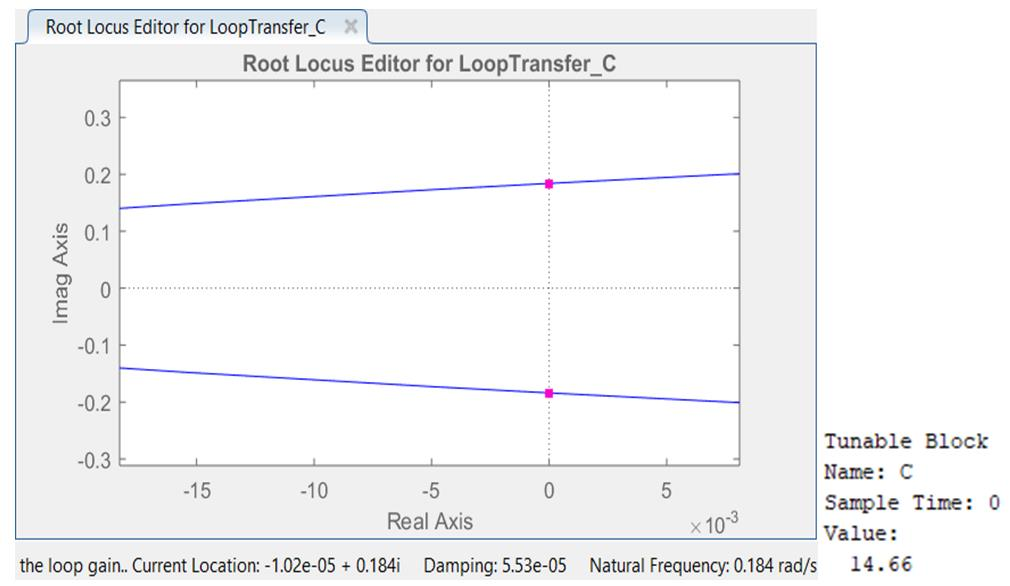
\includegraphics[width=0.8\textwidth]{z2_14}
  \caption{GMK karakteristika stvarnog sistema sa polovima u zatvorenom na imaginarnoj osi, pri čemu je dobiveno pojačanje od $k_{rkrit}=14.66$ (slika u donjem desnom uglu)}
  \label{fig:z2_14}
\end{figure}

\begin{figure} [H]
  \centering
  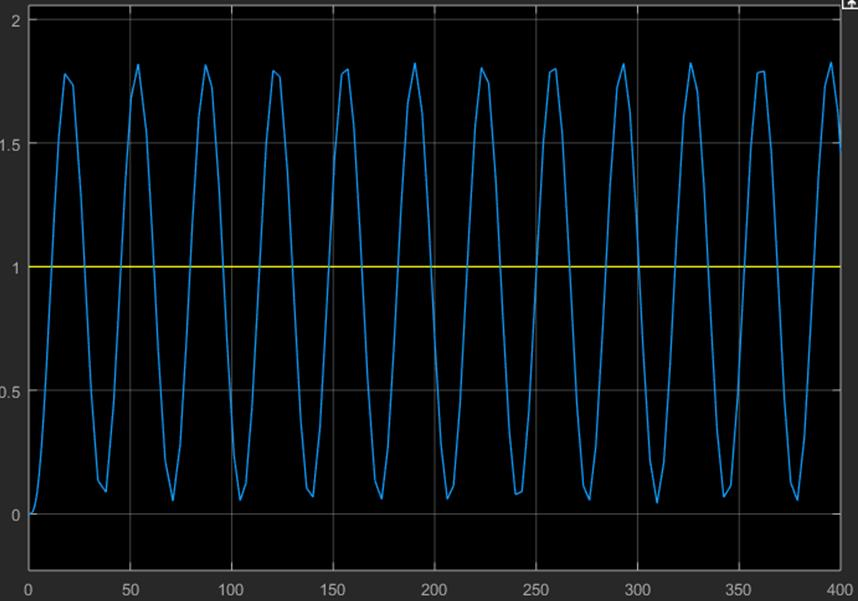
\includegraphics[width=0.8\textwidth]{z2_15}
  \caption{Simulirani odziv na step za dobiveno kritično pojačanje  $k_{rkrit}=14.66$}
  \label{fig:z2_15}
\end{figure}


Simuliranjem odziva na step za dobiveno kritično pojačanje $k_{rkrit}=14.66$, dobijamo stabilne oscilacije (slika \ref{fig:z2_15}) na izlazu perioda $T_{krit}=34.166s$. 


\textbf{e)} Potrebno je podesiti parametre za tri vrste regulacije (P, PI, PID) na osnovu Ziegler-Nichols metode za stvarni sistem. Način podešavanja na osnovu pronađenih vrijednosti $k_{rkrit}=14.66$ i $T_{krit}=34.166s$ je dat u tabeli u prvom zadatku. 

Primjenom ove tabele dobijamo sljedeće rezultate:

\textbf{P regulator: $K_p=8.063$ }(slika \ref{fig:z2_16})
 
\begin{figure} [H]
  \centering
  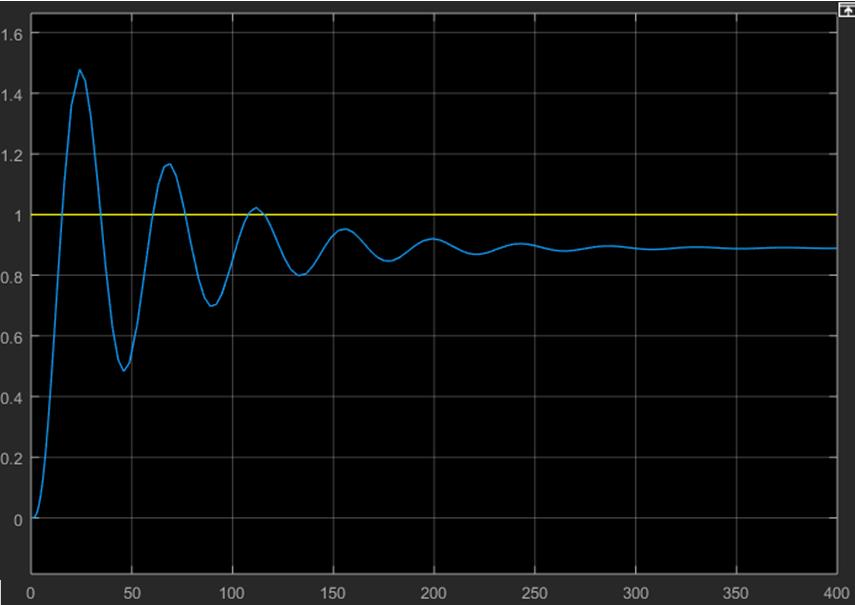
\includegraphics[width=0.8\textwidth]{z2_16}
  \caption{Odziv zatvorenog sistema sa P regulatorom dobivenim Ziegler-Nichols metodom}
  \label{fig:z2_16}
\end{figure}

\textbf{PI regulator: $K_p=5.131, T_i=42.7075$} (slika \ref{fig:z2_17})

\begin{figure} [H]
  \centering
  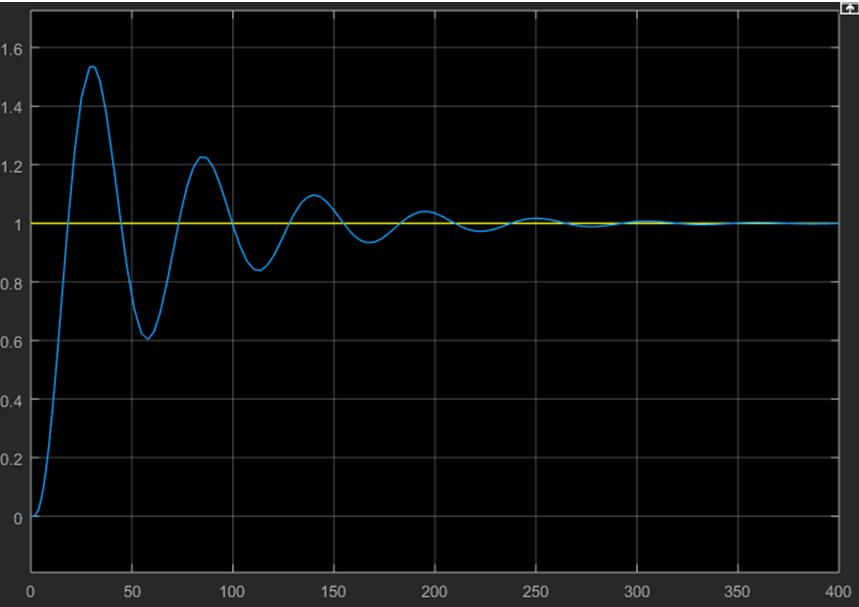
\includegraphics[width=0.8\textwidth]{z2_17}
  \caption{Odziv zatvorenog sistema sa PI regulatorom dobivenim Ziegler-Nichols metodom}
  \label{fig:z2_17}
\end{figure}

\textbf{PID regulator: $K_p=8.796, T_i=27.3328, T_d=6.8332$} (slika \ref{fig:z2_18})
 
\begin{figure} [H]
  \centering
  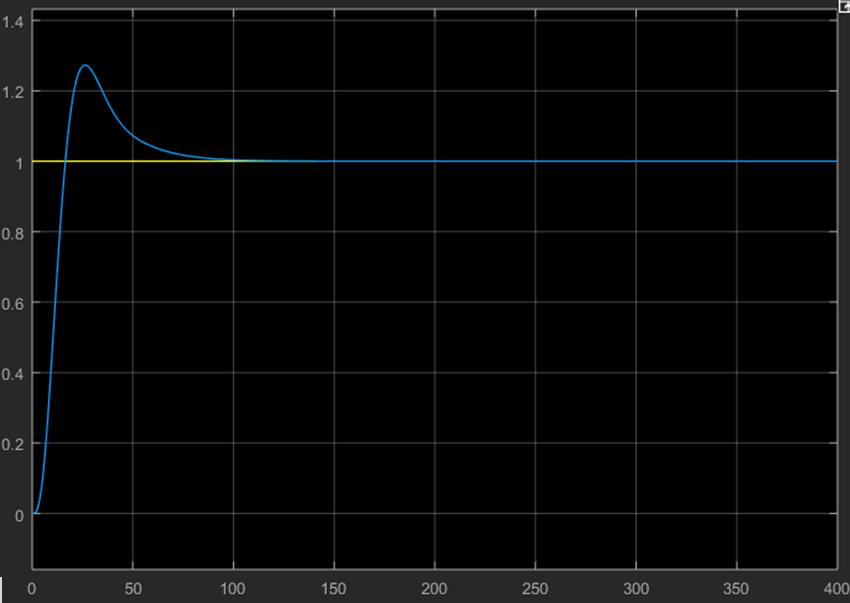
\includegraphics[width=0.8\textwidth]{z2_18}
  \caption{Odziv zatvorenog sistema sa PID regulatorom dobivenim Ziegler-Nichols metodom}
  \label{fig:z2_18}
\end{figure}

\textbf{f)} Potrebno je podesiti parametre za tri vrste regulacije (P, PI, PID) na osnovu Ziegler-Nichols metode za aproksimirani sistem. Način podešavanja je dat u tabeli u prvom zadatku.

Kako je prenosna funkcija aproksimiranog sistema (izračunato pod a)) data kao:
	\[G_{ident} (s)=\frac{1}{49.58s+1} e^{-8.5s}\]

Tako je: $t_z=8.5$, $t_a=49.58$, $K_s=1$. Na osnovu ovih parametara i tabele iz koje se određuju parametri P, PI i PID regulatora (slika \ref{fig:z2_19}) su dobiveni sljedeći rezultati:

\textbf{P regulator: $K_p=5.8329$ (slika \ref{fig:z2_19})}
 
\begin{figure} [H]
  \centering
  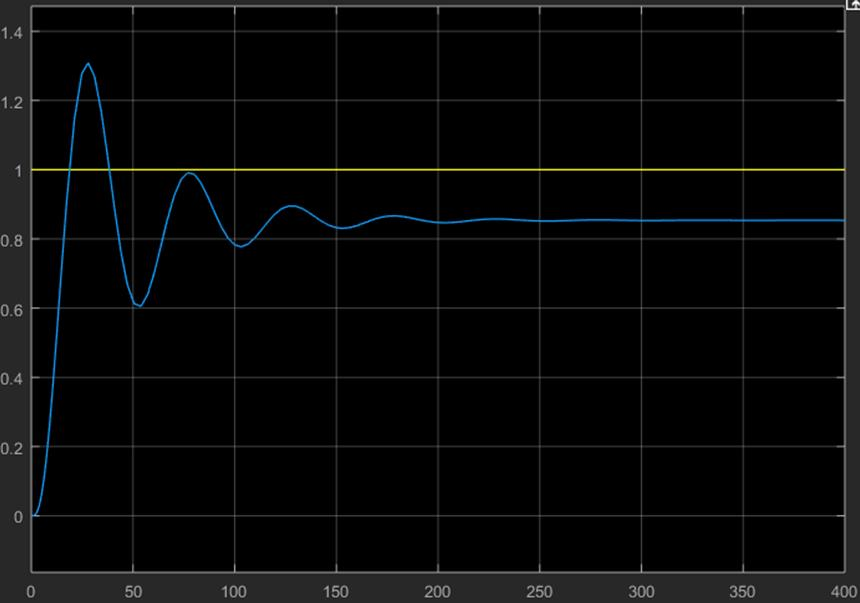
\includegraphics[width=0.8\textwidth]{z2_19}
  \caption{Odziv zatvorenog sistema sa P regulatorom dobivenim Ziegler-Nichols metodom}
  \label{fig:z2_19}
\end{figure}

\textbf{PI regulator: $K_p=5.2496, T_i=28.305$} (slika \ref{fig:z2_20})
 
\begin{figure} [H]
  \centering
  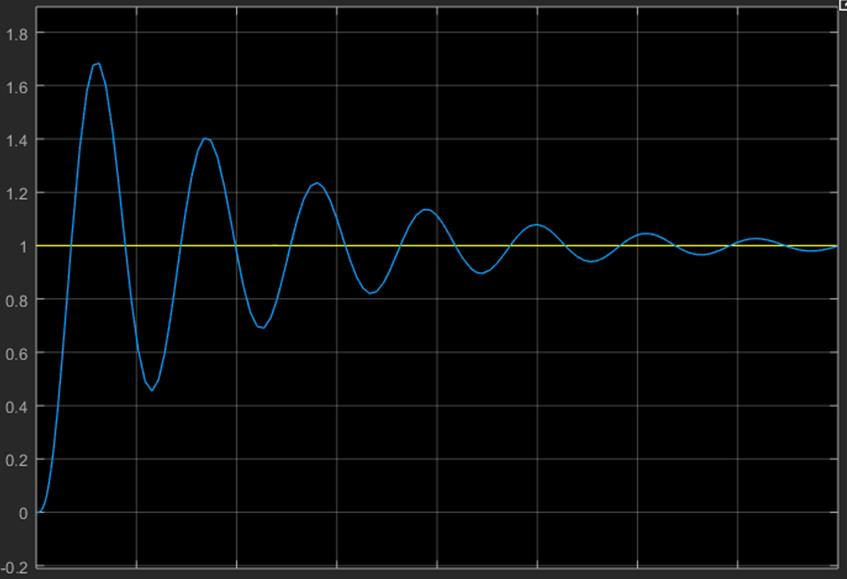
\includegraphics[width=0.8\textwidth]{z2_20}
  \caption{Odziv zatvorenog sistema sa PI regulatorom dobivenim Ziegler-Nichols metodom}
  \label{fig:z2_20}
\end{figure}

\textbf{PID regulator: $K_p=6.9995, T_i=17, T_d=4.25$} (slika \ref{fig:z2_21})

\begin{figure} [H]
  \centering
  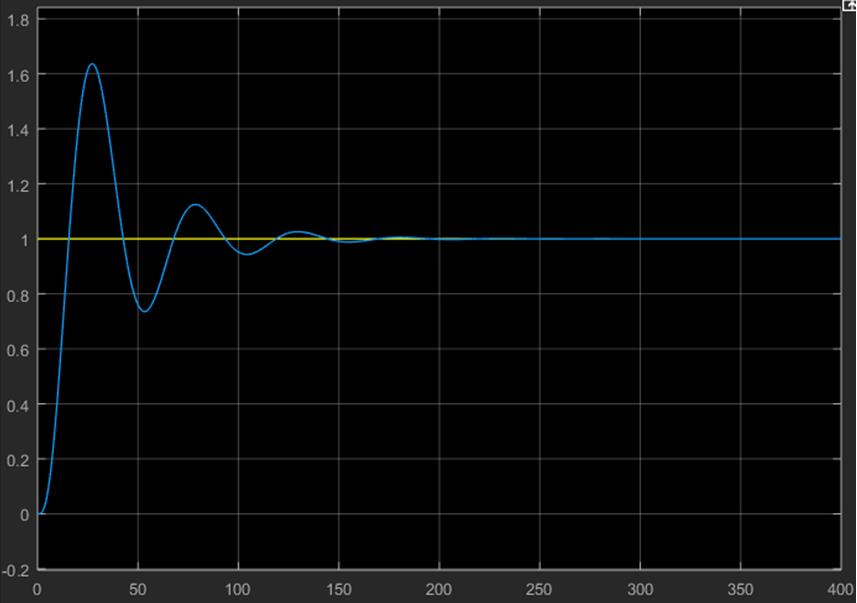
\includegraphics[width=0.8\textwidth]{z2_21}
  \caption{Odziv zatvorenog sistema sa PID regulatorom dobivenim Ziegler-Nichols metodom}
  \label{fig:z2_21}
\end{figure}
 
\textbf{g)} Potrebno je podesiti parametre za tri vrste regulacije (P, PI, PID) na osnovu Cohen-Coon metode za aproksimirani sistem. Način podešavanja je dat u tabeli u prvom zadatku.  Parametri potrebni za izračunavanje parametara P, PI i PID regulatora su dobiveni u stavci pod f) i iznose: $t_z=2.67, t_a=16.66, K_s=0.3555$. Na osnovu ovih parametara dobiveni su sljedeći rezultati:

\textbf{P regulator: $K_p=6.1663$} (slika \ref{fig:z2_22})

\begin{figure} [H]
  \centering
  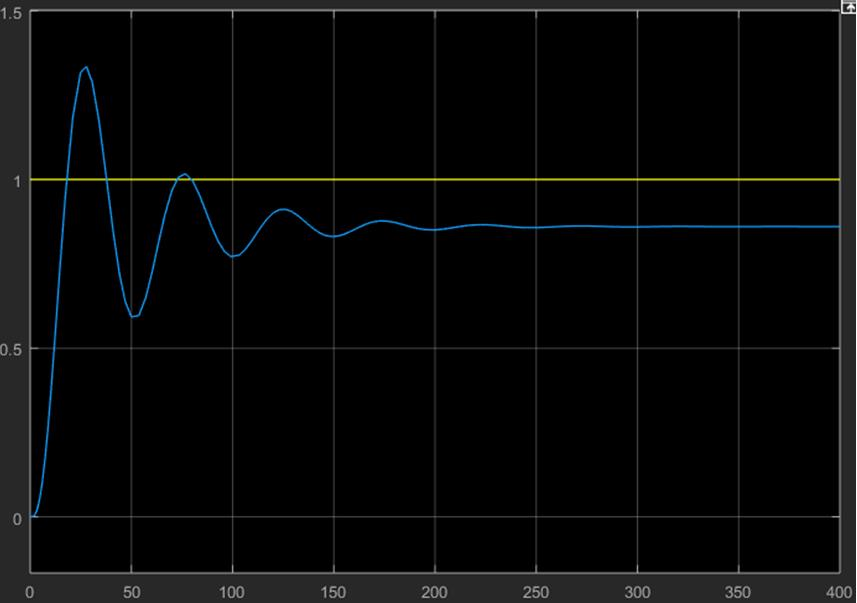
\includegraphics[width=0.8\textwidth]{z2_22}
  \caption{Odziv zatvorenog sistema sa P regulatorom dobivenim Cohen-Coon metodom}
  \label{fig:z2_22}
\end{figure}

\textbf{PI regulator: $K_p=5.333, T_i=19.8998$} (slika \ref{fig:z2_23})

\begin{figure} [H]
  \centering
  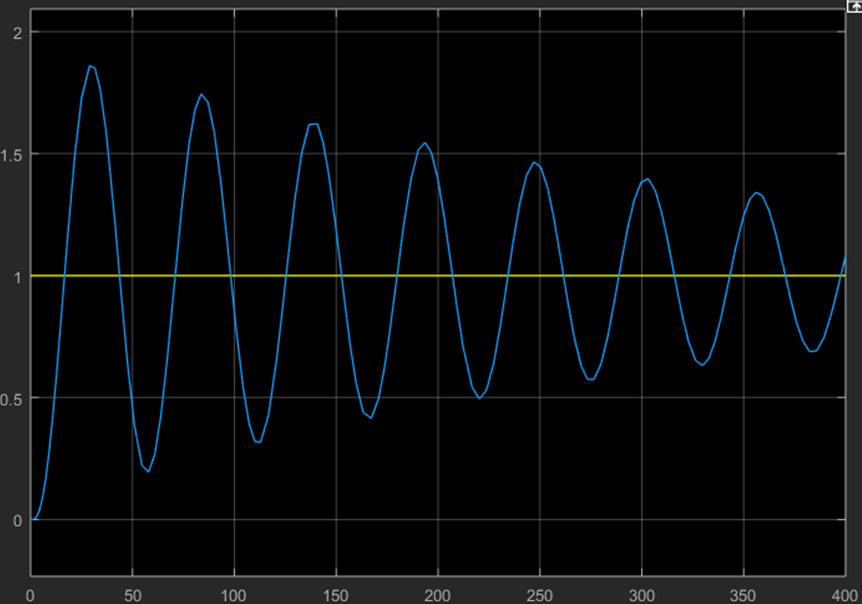
\includegraphics[width=0.8\textwidth]{z2_23}
  \caption{Odziv zatvorenog sistema sa PI regulatorom dobivenim Cohen-Coon metodom}
  \label{fig:z2_23}
\end{figure} 

\textbf{PID regulator: $K_p=8.0273, T_i=19.5347, T_d=2.9975$} (slika \ref{fig:z2_24})

\begin{figure} [H]
  \centering
  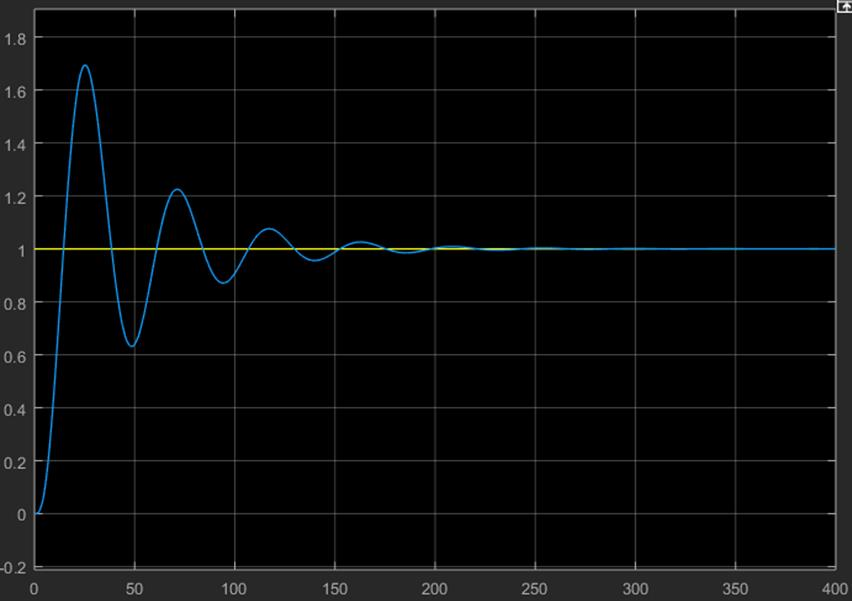
\includegraphics[width=0.8\textwidth]{z2_24}
  \caption{Odziv zatvorenog sistema sa PID regulatorom dobivenim Cohen-Coon metodom}
  \label{fig:z2_24}
\end{figure}

\textbf{h)} U ovom dijelu je potrebno uporediti P, PI i PID regulatore dobivene različitim metodama u stavkama e), f) i g). Što se tiče P regulatora, metode zasnovane na aproksimaciji sistema sistemom prvog reda sa čistim transportnim kašnjenjem su dale bolje rezultate od Ziegler-Nichols metode koja podrazumijeva dovođenje sistema na granicu stabilnosti. Što se tiče PI regulatora, najbolji rezultat je dala metoda Ziegler-Nichols koja podrazumijeva dovođenje sistema na granicu stabilnosti. Ovom metodom su dobiveni najkraće vrijeme smirenja, najmanji preskok. Nakon ove metode slijedi Ziegler-Nichols metoda koja podrazumijeva identifikaciju sistema. Ova metoda je dala nešto veće vrijeme smirenja te veći preskok. Najgore rezultate za PI regulator je dala metoda Cohen-Coon koja je dala još veće vrijeme smirenja te veći prvi preskok. Što se tiče PID regulatora, najbolji rezultat je ponovo dala metoda Ziegler-Nichols koja podrazumijeva dovođenje sistema na granicu stabilnosti. Ovom metodom su dobiveni najkraće vrijeme smirenja, najmanji preskok, dok su oscilacije eliminisane. Nakon ove metode slijedi Ziegler-Nichols metoda koja podrazumijeva identifikaciju sistema. Ova metoda je dala veće vrijeme smirenja, veći preskok, a nije eliminisala oscilacije. Najgore rezultate je dala metoda Cohen-Coon koja ima još veći preskok, veće vrijeme smirenja te više oscilacija od Ziegler-Nichols metode koja se zasniva na identifikaciji sistema.

\textbf{i)} Potrebno je vidjeti kako se sistem ponaša kada dodamo smetnju prije upravljanog objekta, tj. simuliramo grešku u aproksimaciji modela sistema. Kao što je navedeno, koriste se parametri iz stavke e) za sva tri regulatora P, PI i PID. Dobiveni su sljedeći rezultati:

\textbf{P regulator: $K_p=8.063$} (slika \ref{fig:z2_25})

\begin{figure} [H]
  \centering
  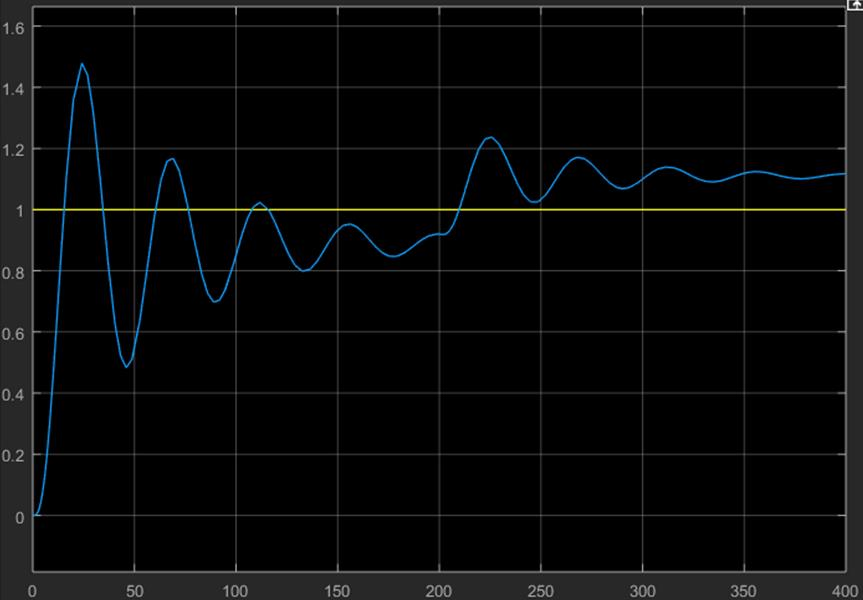
\includegraphics[width=0.8\textwidth]{z2_25}
  \caption{Odziv zatvorenog sistema sa P regulatorom dobivenim Ziegler-Nichols metodom}
  \label{fig:z2_25}
\end{figure}

\textbf{PI regulator: $K_p=5.131, T_i=42.7075$} (slika \ref{fig:z2_26})

\begin{figure} [H]
  \centering
  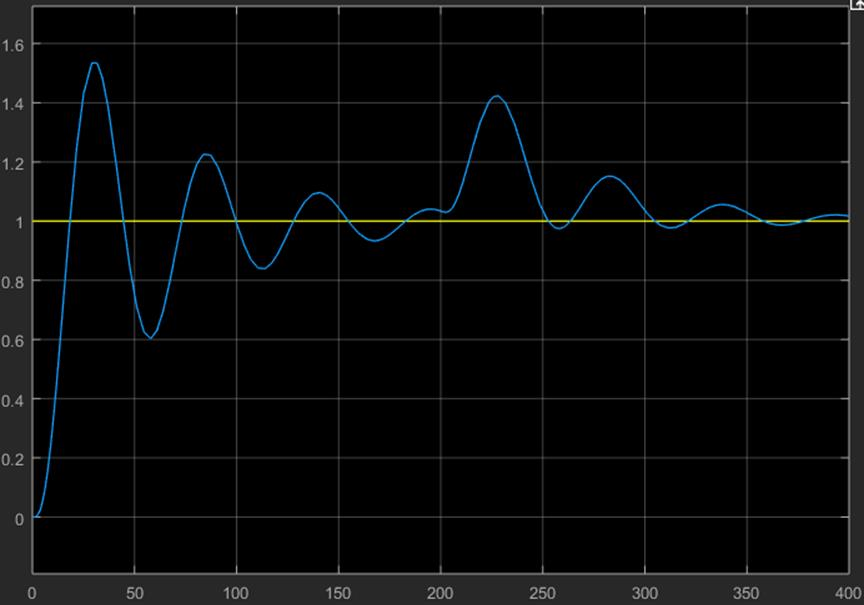
\includegraphics[width=0.8\textwidth]{z2_26}
  \caption{Odziv zatvorenog sistema sa PI regulatorom dobivenim Ziegler-Nichols metodom}
  \label{fig:z2_26}
\end{figure}

\textbf{PID regulator: $K_p=8.796, T_i=27.3328, T_d=6.8332$} (slika \ref{fig:z2_27})

\begin{figure} [H]
  \centering
  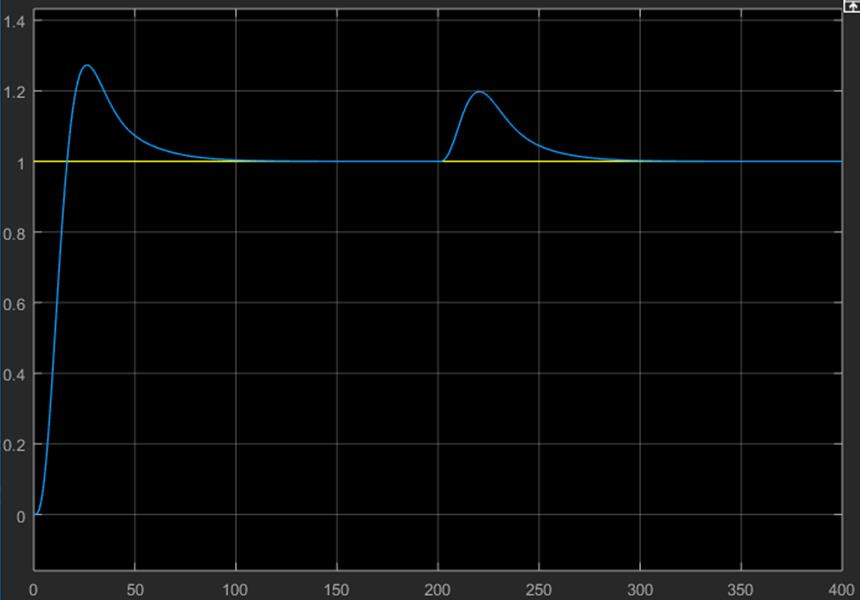
\includegraphics[width=0.8\textwidth]{z2_27}
  \caption{Odziv zatvorenog sistema sa PID regulatorom dobivenim Ziegler-Nichols metodom}
  \label{fig:z2_27}
\end{figure}

Step smetnja koja je dodana ispred objekta kojim se upravlja je dodana u trenutku t=200s i njena amplituda je 2. Možemo vidjeti da sam P regulator ne reaguje dobro na dodanu smetnju jer samo pomjeri grešku u stacionarnom stanju na neku drugu vrijednost. PI regulator se dobro nosi sa ovom smetnjom jer I komponenta na kraju ponovo eliminiše grešku u stacionarnom stanju. PID regulator se također dobro nosi sa ovom smetnjom, jer I komponenta eliminiše grešku u stacionarnom stanju, dok D komponenta smanjuje oscilacije i smanjuje amplitudu preskoka.
























